\documentclass{beamer}

\usetheme{Madrid}
\usecolortheme{default}

% Configure footer to show only page number
\setbeamertemplate{footline}[frame number]
\setbeamertemplate{navigation symbols}{}

\usepackage{amsmath}
\usepackage{amssymb}
\usepackage{graphicx}
\usepackage{tikz}
\usepackage{pgfplots}
\pgfplotsset{compat=1.18}
\usepackage{algorithm}
\usepackage{algpseudocode}
\usepackage{siunitx}

% % ---- IITH logo in top-right corner on all slides ----
% \addtobeamertemplate{frametitle}{}{%
%     \begin{textblock*}{0cm}(0.88\textwidth,-0.9cm)
%         \hfill \includegraphics[width=0.9cm]{iith_logo.png}
%     \end{textblock*}
% }


\title{Hierarchical Control of \\Cooperative Quadrotor Payload Transport}
\author{
    A 6-DOF Rigid Body Dynamics Simulation\\ with Geometric Attitude Control \\
    \vspace{0.5cm}
    \small \textbf{Term Project for Control Systems Design (ME5780)} \\
    \vspace{0.5cm}
    \normalsize
    Arkaprabha Sinha Roy (AI25MTECH12001) \\
    Rehbar Khan (ME25MTECH11015) \\
    S. Chinnikrishna Yadav (ME25MTECH12005) \\
    Vikram Kumar Anand (ME25MTECH14011)
}
\institute{Indian Institute of Technology Hyderabad}
\date{\small November 2025}

\begin{document}

% Slide 1: Title
\frame{\titlepage}

% Slides 2-3: Introduction
\begin{frame}{Introduction: Motivation}
\textbf{Cooperative Aerial Manipulation}
\begin{itemize}
    \item Multi-drone systems for heavy payload transport
    \item Applications: construction, disaster response, logistics
    \item Advantages: exceeds individual capacity, redundancy, flexibility
\end{itemize}

\vspace{0.5cm}
\textbf{Key Challenges}
\begin{itemize}
    \item Coupled dynamics in closed kinematic chain
    \item Underactuated quadrotor systems (4 inputs, 6 DOF)
    \item Nonlinear SO(3) attitude dynamics
    \item Thrust allocation with saturation constraints
    \item Model uncertainty and disturbances
\end{itemize}
\end{frame}

\begin{frame}{Introduction: Contributions}
\begin{enumerate}
    \item Complete 6-DOF rigid body simulation framework
    \begin{itemize}
        \item Newton-Euler dynamics with Rodrigues integration
        \item Point mass drone modeling
    \end{itemize}
    \item Hierarchical control architecture
    \begin{itemize}
        \item Geometric attitude control on SO(3)
        \item PID position regulation
    \end{itemize}
    \item Multi-phase trajectory planning (7 phases)
    \begin{itemize}
        \item Quintic polynomial profiles with C$^2$ continuity
    \end{itemize}
    \item Realistic DJI Matrice 300 RTK modeling
    \item Comprehensive noise modeling (mass, thrust, attachment, wind)
    \item JSON-based real-time telemetry system
\end{enumerate}
\end{frame}

% Slide 4: System Model - Payload Dynamics
\begin{frame}{System Model: Payload Dynamics}
\textbf{6-DOF Rigid Body Equations}

Translational dynamics:
\[
m\ddot{\mathbf{x}} = \sum_{i=1}^{4} \mathbf{F}_i + m\mathbf{g} + \mathbf{F}_{\text{wind}}
\]

Rotational dynamics (Newton-Euler on $\mathbb{R}^3$):
\[
\mathbf{I}\dot{\boldsymbol{\omega}} + \boldsymbol{\omega} \times \mathbf{I}\boldsymbol{\omega} = \boldsymbol{\tau}_{\text{ext}} = \sum_{i=1}^{4} \mathbf{r}_i \times \mathbf{F}_i
\]

Attitude kinematics on SO(3):
\[
\dot{\mathbf{R}} = \mathbf{R} \, \widehat{\boldsymbol{\omega}}, \quad \widehat{\boldsymbol{\omega}} = \begin{bmatrix} 0 & -\omega_z & \omega_y \\ \omega_z & 0 & -\omega_x \\ -\omega_y & \omega_x & 0 \end{bmatrix}
\]

\textbf{Cubic Payload:} $a = \SI{0.25}{m}$, $m = \SI{10}{kg}$, $\mathbf{I} = \frac{ma^2}{6}\mathbf{I}_3$
\end{frame}

% Slide 5: System Model - Drone Dynamics
\begin{frame}{System Model: Drone Dynamics}
\textbf{Point Mass Model with Actuator Dynamics}

Drone position (body-frame attachment):
\[
\mathbf{p}_i = \mathbf{x} + \mathbf{R}\mathbf{r}_i, \quad \dot{\mathbf{p}}_i = \dot{\mathbf{x}} + \dot{\mathbf{R}}\mathbf{r}_i = \dot{\mathbf{x}} + \mathbf{R}(\widehat{\boldsymbol{\omega}}\mathbf{r}_i)
\]

Constraint force (cable):
\[
\mathbf{F}_i = -\mathbf{T}_i, \quad \text{(Newton's 3rd law)}
\]

First-order motor lag:
\[
\dot{\mathbf{T}}_i = \frac{1}{\tau_m}(\mathbf{T}_{i,\text{cmd}} - \mathbf{T}_i), \quad \tau_m = \SI{0.2}{s}
\]

\textbf{DJI Matrice 300 RTK:} $m_d = \SI{6.3}{kg}$, $T_{\max} = \SI{126}{N}$
\end{frame}

% Slide 6: Noise and Disturbances
\begin{frame}{Noise and Disturbances}
\textbf{Realistic Operating Conditions}

\begin{table}[h]
\centering
\begin{tabular}{lc}
\hline
\textbf{Source} & \textbf{Magnitude} \\
\hline
Mass variance & 2\% of drone mass \\
Thrust noise & 5\% of thrust magnitude \\
Attachment point error & 1\% of payload size \\
Wind baseline velocity & \SI{0.5}{m/s} \\
Wind gust intensity & \SI{0.3}{m/s/\sqrt{s}} \\
Drag coefficient & $C_d = 1.0$ \\
\hline
\end{tabular}
\end{table}

\vspace{0.3cm}
Wind force model:
\[
\mathbf{F}_{\text{wind}} = \frac{1}{2}\rho_{\text{air}} C_d A \|\mathbf{v}_{\text{wind}}\| \mathbf{v}_{\text{wind}}
\]
\end{frame}

% Slide 7: Block Diagram
\begin{frame}{Control Architecture: Block Diagram}
\begin{columns}[c]

  % Left column: text
  \begin{column}{0.48\textwidth}
    \textbf{Hierarchical Structure}
    \vspace{6pt}
    \begin{itemize}
      \item \textbf{Outer loop:} Position control (PID)
      \item \textbf{Inner loop:} Attitude control (Geometric control on $SO(3)$)
    \end{itemize}
  \end{column}

  % Right column: image (with fallback)
  \begin{column}{0.52\textwidth}
    \centering
    % If the image file exists, include it; otherwise show a placeholder box
    \IfFileExists{diagram-4x.png}{%
      \includegraphics[width=\linewidth,keepaspectratio]{diagram-4x.png}%
    }{%
      \fbox{%
        \parbox[c][0.45\textwidth][c]{0.9\linewidth}{%
          \centering
          \textbf{diagram-4x.png not found}\\
          Upload the image to your Overleaf project or change the filename.
        }%
      }%
    }
  \end{column}

\end{columns}
\end{frame}

% Slide 8: Position Control
\begin{frame}{Position Control: PID}
\textbf{Outer-loop translational control}

Position and velocity tracking errors:
\[
\mathbf{e}_p = \mathbf{x} - \mathbf{x}_d, \quad \mathbf{e}_v = \dot{\mathbf{x}} - \dot{\mathbf{x}}_d, \quad \mathbf{e}_i = \int_0^t \mathbf{e}_p \, d\tau
\]

PID control law (feedforward + feedback):
\[
\mathbf{F}_d = m(\ddot{\mathbf{x}}_d - \mathbf{g} - K_p \mathbf{e}_p - K_d \mathbf{e}_v - K_i \mathbf{e}_i)
\]

\textbf{Ziegler-Nichols Tuning:}
\[
K_p = 0.8 K_u, \quad K_d = 0.1 K_u T_u, \quad K_i = 0
\]
where $K_{u,xy} = 0.08 T_{\max}$, $K_{u,z} = 0.12 T_{\max}$, $T_u = \SI{3.5}{s}$

Anisotropic gains: vertical $\neq$ horizontal (different dynamics)
\end{frame}

% Slide 9: Geometric Attitude Control
\begin{frame}{Geometric Attitude Control on SO(3)}
\textbf{Inner-loop rotational control (Lee et al., 2010)}

Desired attitude from thrust direction:
\[
\mathbf{b}_3 = \frac{\mathbf{F}_d}{\|\mathbf{F}_d\|}, \quad \mathbf{b}_1 = \frac{\mathbf{b}_2 \times \mathbf{b}_3}{\|\mathbf{b}_2 \times \mathbf{b}_3\|}, \quad \mathbf{R}_d = [\mathbf{b}_1 \, \mathbf{b}_2 \, \mathbf{b}_3]
\]

Attitude error on Lie algebra $\mathfrak{so}(3)$ (vee map):
\[
\mathbf{e}_R = \frac{1}{2}(\mathbf{R}_d^T \mathbf{R} - \mathbf{R}^T \mathbf{R}_d)^\vee \in \mathbb{R}^3
\]

Control torque with gyroscopic compensation:
\[
\boldsymbol{\tau}_d = -K_R \mathbf{e}_R - K_\omega (\boldsymbol{\omega} - \mathbf{R}^T\mathbf{R}_d\boldsymbol{\omega}_d) + \boldsymbol{\omega} \times \mathbf{I}\boldsymbol{\omega}
\]

High gains: $K_R = K_\omega = 4T_{\max}$ (fast attitude tracking)
\end{frame}

% Slide 10: Thrust Allocation
\begin{frame}{Thrust Allocation}
\textbf{Least-squares with zero net force constraint}

Wrench mapping (force $\to$ torque):
\[
\boldsymbol{\tau} = \sum_{i=1}^{4} \mathbf{r}_i \times \mathbf{F}_i = \sum_{i=1}^{4} \widehat{\mathbf{r}}_i \mathbf{F}_i
\]

Constrained optimization:
\[
\min_{\{\delta\mathbf{F}_i\}} \left\|\begin{bmatrix} \sum_i \delta\mathbf{F}_i \\ \sum_i \widehat{\mathbf{r}}_i \delta\mathbf{F}_i \end{bmatrix} - \begin{bmatrix} \mathbf{0} \\ \boldsymbol{\tau}_d \end{bmatrix}\right\|^2
\]

Matrix form: $\mathbf{A} \delta\mathbf{F} = \mathbf{b}$, where
\[
\mathbf{A} = \begin{bmatrix} \mathbf{I}_3 & \mathbf{I}_3 & \mathbf{I}_3 & \mathbf{I}_3 \\ \widehat{\mathbf{r}}_1 & \widehat{\mathbf{r}}_2 & \widehat{\mathbf{r}}_3 & \widehat{\mathbf{r}}_4 \end{bmatrix} \in \mathbb{R}^{6 \times 12}
\]

Solution: $\delta\mathbf{F} = \mathbf{A}^\dagger \mathbf{b}$ (Moore-Penrose pseudoinverse)
\end{frame}

% Slide 11: Trajectory Generation
\begin{frame}{Trajectory Generation}
\textbf{Quintic Polynomial Interpolation (C$^2$ smooth)}

Boundary value problem for each axis:
\[
s(t) = a_0 + a_1 t + a_2 t^2 + a_3 t^3 + a_4 t^4 + a_5 t^5
\]

Constraints at $t=0$ and $t=T$:
\[
s(0) = s_0, \; \dot{s}(0) = v_0, \; \ddot{s}(0) = a_0, \quad s(T) = s_f, \; \dot{s}(T) = v_f, \; \ddot{s}(T) = a_f
\]

\textbf{7-Phase Profile:} takeoff $\to$ hover $\to$ translate $\to$ hover $\to$ translate $\to$ hover $\to$ land

Feedforward acceleration from trajectory:
\[
\mathbf{a}_d(t) = \ddot{\mathbf{x}}_d(t) = [12a_4 t^2 + 6a_3 t + 2a_2]
\]
\end{frame}

% Slide 22: Implementation Details
\begin{frame}{Implementation Details}
\textbf{Numerical Integration on SO(3)}

Rodrigues formula (exponential map):
\[
\mathbf{R}_{k+1} = \mathbf{R}_k \exp(\widehat{\boldsymbol{\omega}}_k \Delta t)
\]

Exponential of skew-symmetric matrix:
\[
\exp(\widehat{\boldsymbol{\omega}} \theta) = \mathbf{I} + \frac{\sin\theta}{\theta}\widehat{\boldsymbol{\omega}} + \frac{1-\cos\theta}{\theta^2}\widehat{\boldsymbol{\omega}}^2
\]
where $\theta = \|\boldsymbol{\omega}\| \Delta t$

\textbf{Advantages:}
\begin{itemize}
    \item Preserves $\mathbf{R} \in \text{SO}(3)$ (no drift, $\det(\mathbf{R})=1$, $\mathbf{R}^T\mathbf{R}=\mathbf{I}$)
    \item Singularity-free (no Euler angles)
    \item Second-order accurate
\end{itemize}

Translational: Semi-implicit Euler, $\Delta t = \SI{0.01}{s}$
\end{frame}

% Slide 12: Parameters
\begin{frame}{Simulation Parameters}
\begin{table}[h]
\centering
\small
\begin{tabular}{ll}
\hline
\textbf{Parameter} & \textbf{Value} \\
\hline
Time step & \SI{0.01}{s} \\
Time scale factor & 0.7 \\
Payload size & \SI{0.25}{m} \\
Payload mass & \SI{10}{kg} \\
Drone mass (each) & \SI{6.3}{kg} \\
Drone max thrust & \SI{126}{N} \\
Motor time constant & \SI{0.2}{s} \\
Gravity & \SI{9.80665}{m/s^2} \\
Air density & \SI{1.225}{kg/m^3} \\
$K_R, K_\omega$ & $4T_{\max}$ \\
$K_{p,xy}$ & $0.064 T_{\max}$ \\
$K_{p,z}$ & $0.096 T_{\max}$ \\
$K_{d,xy}$ & $0.028 T_{\max}$ \\
$K_{d,z}$ & $0.042 T_{\max}$ \\
\hline
\end{tabular}
\end{table}
\end{frame}

% Slides 13-15: Experiment 0
\begin{frame}{Experiment 0: Ideal Baseline}
\textbf{Quintic Trajectory with Ideal Conditions}

\vspace{0.5cm}
\textbf{Objective:}
\begin{itemize}
    \item Validate controller performance under perfect conditions
    \item Establish baseline for comparison
\end{itemize}

\vspace{0.5cm}
\textbf{Setup:}
\begin{itemize}
    \item No noise, no disturbances, no transient effects
    \item Perfect mass, attachment, and thrust model
    \item Quintic polynomial trajectory with C$^2$ continuity
\end{itemize}

\vspace{0.5cm}
\textbf{Methodology:}
\begin{itemize}
    \item 7-phase mission: takeoff $\rightarrow$ hover $\rightarrow$ translate E $\rightarrow$ hover $\rightarrow$ translate N $\rightarrow$ hover $\rightarrow$ land
    \item Target: (10m E, 10m N, 5m altitude)
\end{itemize}
\end{frame}

\begin{frame}{Experiment 0: Plots}
\begin{center}

\includegraphics[width=0.95\textwidth]{expts/0/com3d.png}
\end{center}
\end{frame}

\begin{frame}{Experiment 0: Plots (continued)}
\begin{columns}
\column{0.5\textwidth}

\includegraphics[width=\textwidth]{expts/0/com.png}
\column{0.5\textwidth}
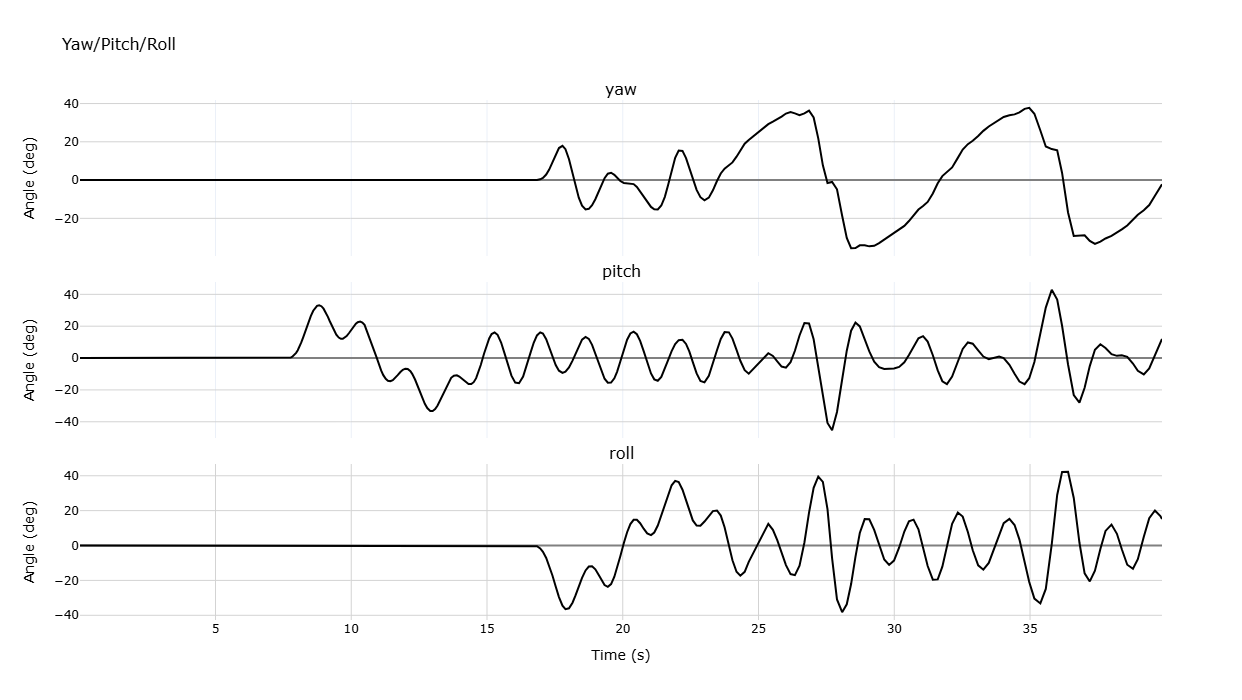
\includegraphics[width=\textwidth]{expts/0/rot.png}
\end{columns}
\end{frame}

\begin{frame}{Experiment 0: Observations}
\textbf{Key Findings:}
\begin{itemize}
    \item Position error $<$ 17 cm throughout mission
    \item Final position: (10.063m N, 10.098m E) --- within 10cm
    \item Attitude excursions $<$ 30° (max yaw during hover)
    \item Impact velocity: 0.35 m/s (safe landing)
\end{itemize}

\vspace{0.5cm}
\textbf{Discussion:}
\begin{itemize}
    \item Controllers perform excellently under ideal conditions
    \item Quintic trajectories provide smooth C$^2$ continuity
    \item Sets performance baseline for disturbance analysis
\end{itemize}
\end{frame}

% Slides 16-18: Experiment 1
\begin{frame}{Experiment 1: No Control with Disturbances}
\textbf{Open-Loop System with Realistic Disturbances}

\vspace{0.5cm}
\textbf{Objective:}
\begin{itemize}
    \item Demonstrate necessity of feedback control
    \item Analyze system instability without controllers
\end{itemize}

\vspace{0.5cm}
\textbf{Setup:}
\begin{itemize}
    \item Transient motor dynamics ($\tau_m = 0.2$s)
    \item Mass variance: 2\%, Thrust noise: 5\%, Attachment error: 1\%
    \item Wind: 0.5 m/s baseline + 0.3 m/s/$\sqrt{s}$ gust intensity
    \item \textbf{Controllers disabled} --- open-loop quintic trajectory only
\end{itemize}

\vspace{0.5cm}
\textbf{Methodology:}
\begin{itemize}
    \item Same trajectory as Experiment 0
    \item Compare divergence without feedback control
\end{itemize}
\end{frame}

\begin{frame}{Experiment 1: Plots}
\begin{center}
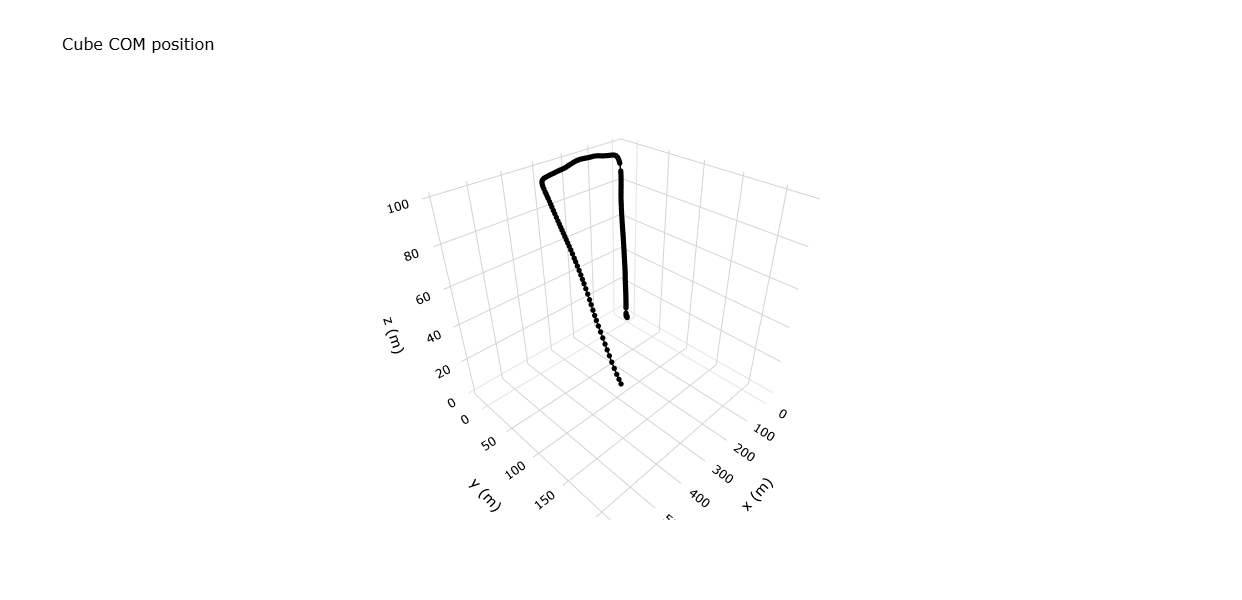
\includegraphics[width=0.95\textwidth]{expts/1/com3d.png}
\end{center}
\end{frame}

\begin{frame}{Experiment 1: Plots (continued)}
\begin{columns}
\column{0.5\textwidth}

\includegraphics[width=\textwidth]{expts/1/com.png}
\column{0.5\textwidth}
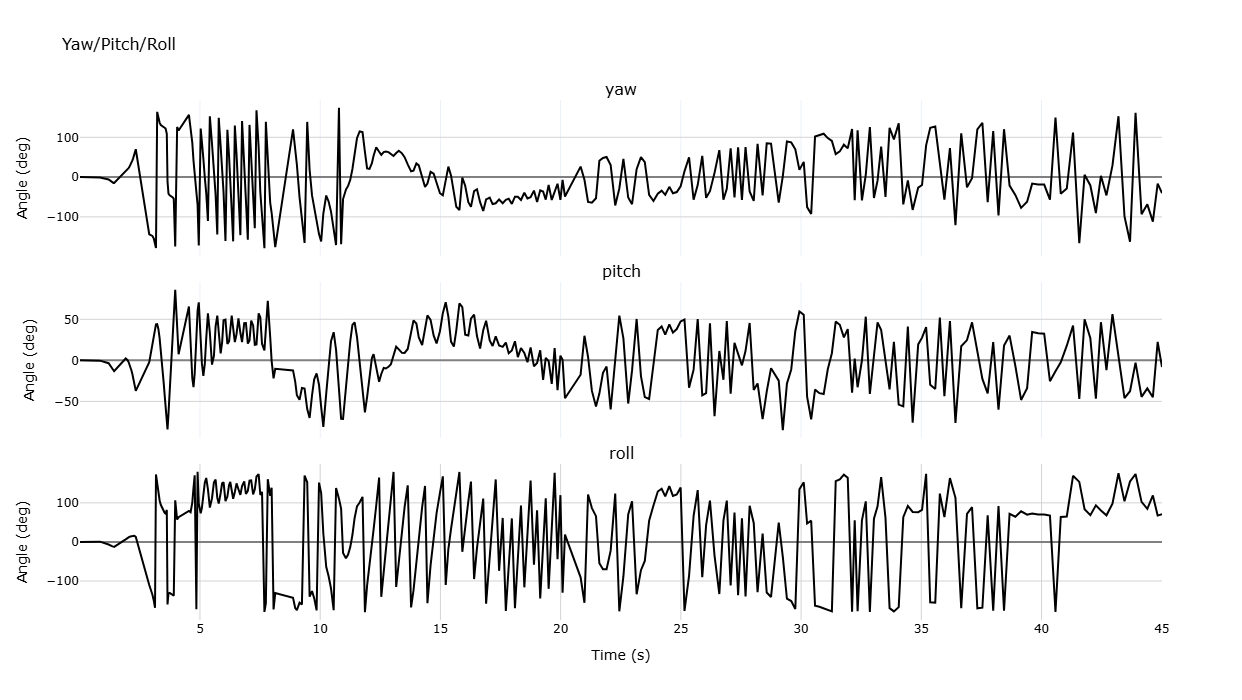
\includegraphics[width=\textwidth]{expts/1/rot.png}
\end{columns}
\end{frame}

\begin{frame}{Experiment 1: Observations}
\textbf{Key Findings:}
\begin{itemize}
    \item \textbf{Catastrophic divergence}: 619m error by end
    \item Final position: (216m N, 589m E, -73m D) --- complete failure
    \item Attitude excursions $>$ 120° --- total instability
    \item System velocity: 32 m/s and increasing
\end{itemize}

\vspace{0.5cm}
\textbf{Discussion:}
\begin{itemize}
    \item Without feedback, small disturbances compound exponentially
    \item Transient motor lag amplifies position errors
    \item Demonstrates critical importance of closed-loop control
    \item Underactuated system inherently unstable under perturbations
\end{itemize}
\end{frame}

% Slides 19-21: Experiment 2
\begin{frame}{Experiment 2: Full Control with Disturbances}
\textbf{Hierarchical Control Under Realistic Conditions}

\vspace{0.5cm}
\textbf{Objective:}
\begin{itemize}
    \item Validate robustness of hierarchical control architecture
    \item Demonstrate disturbance rejection capabilities
\end{itemize}

\vspace{0.5cm}
\textbf{Setup:}
\begin{itemize}
    \item Identical disturbances as Experiment 1
    \item Transient motor dynamics, mass/thrust/attachment errors, wind
    \item \textbf{All controllers enabled}: PID position + geometric attitude
    \item Quintic trajectory planning with feedback
\end{itemize}

\vspace{0.5cm}
\textbf{Methodology:}
\begin{itemize}
    \item Same mission profile as baseline
    \item Evaluate controller performance under realistic conditions
\end{itemize}
\end{frame}

\begin{frame}{Experiment 2: Plots}
\begin{center}
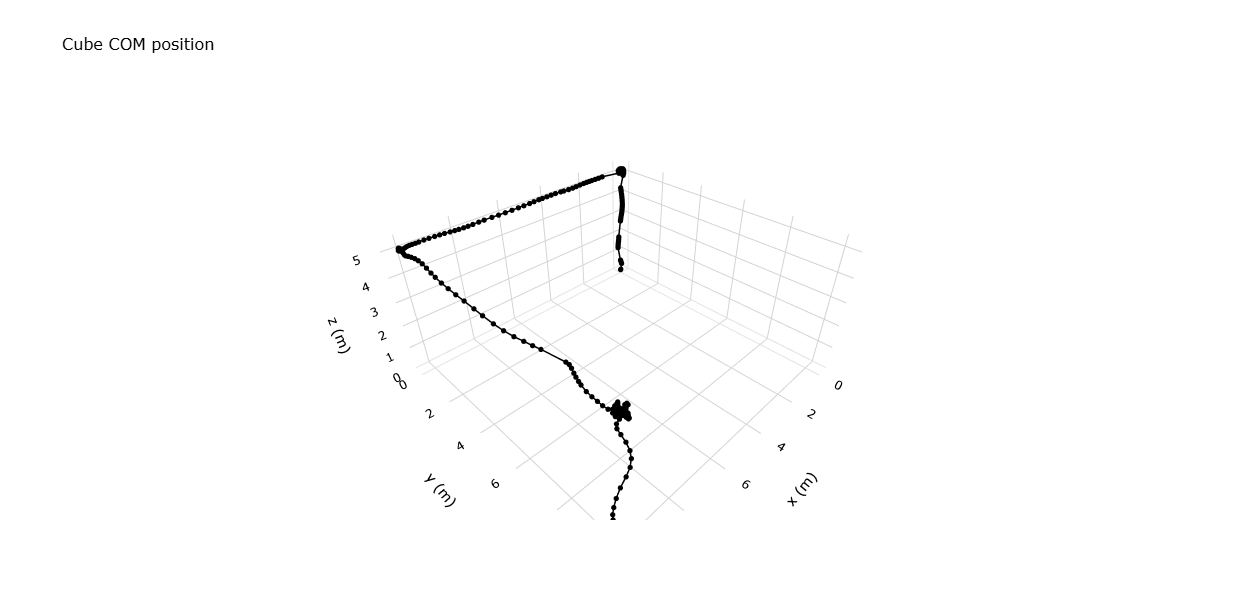
\includegraphics[width=0.95\textwidth]{expts/2/com3d.png}
\end{center}
\end{frame}

\begin{frame}{Experiment 2: Plots (continued)}
\begin{columns}
\column{0.5\textwidth}
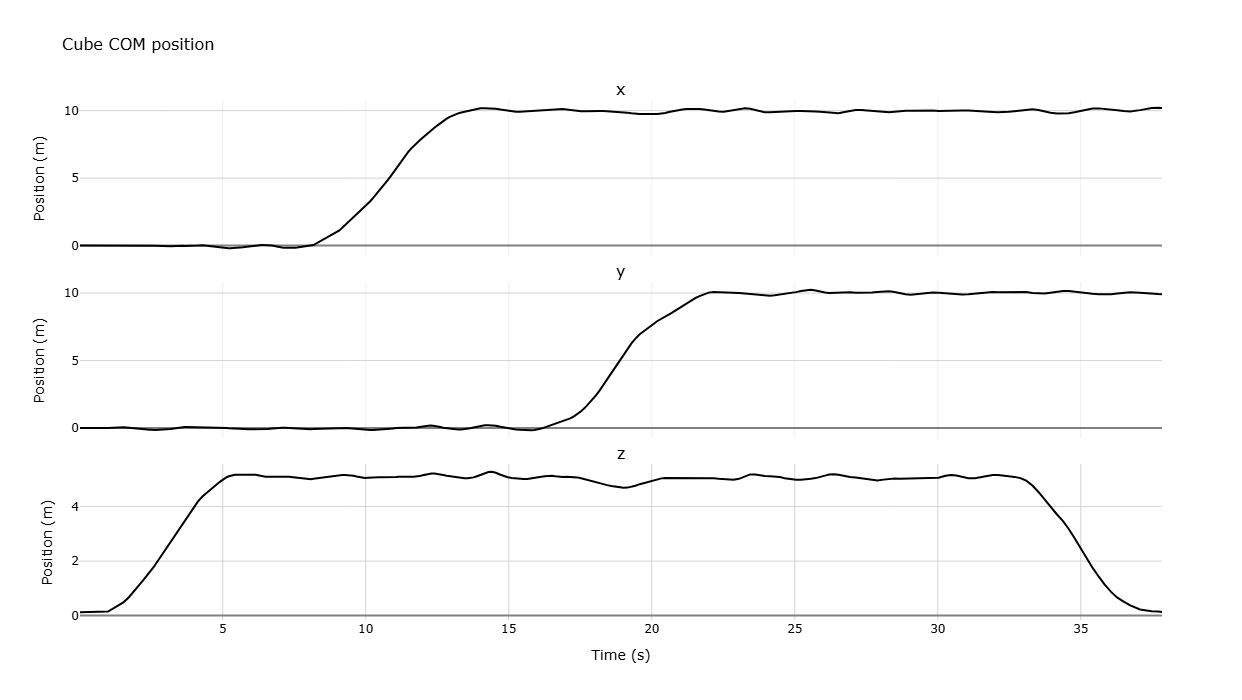
\includegraphics[width=\textwidth]{expts/2/com.png}
\column{0.5\textwidth}
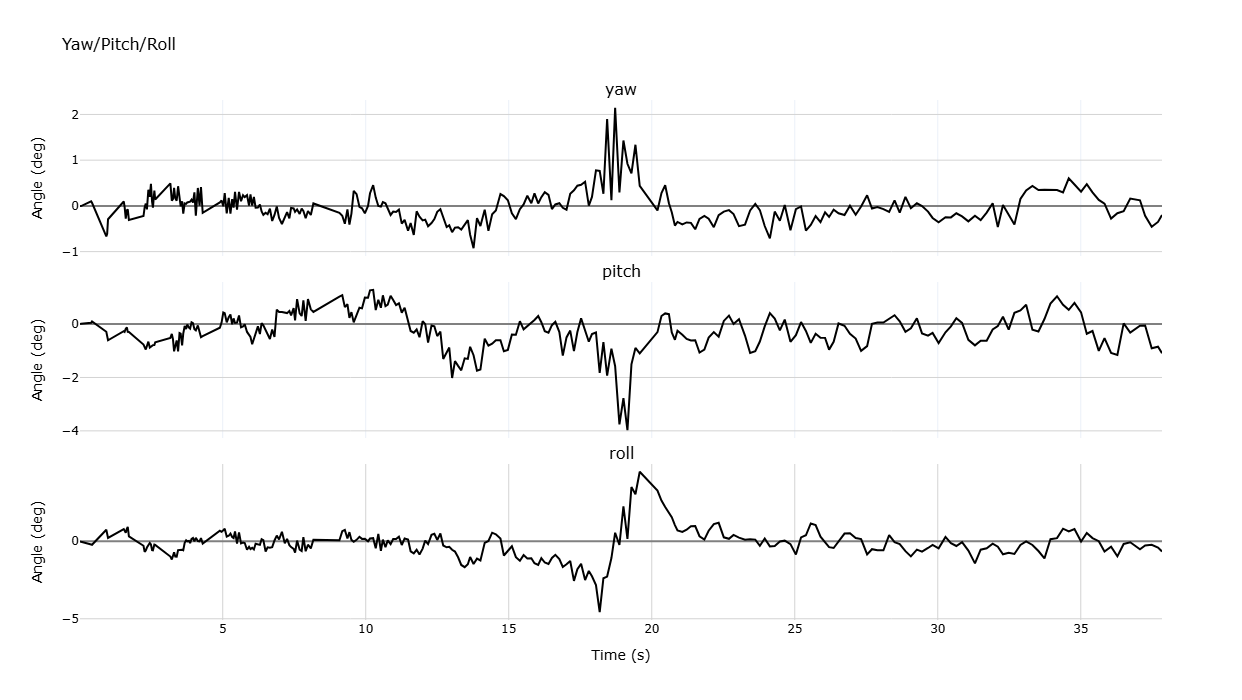
\includegraphics[width=\textwidth]{expts/2/rot.png}
\end{columns}
\end{frame}

\begin{frame}{Experiment 2: Observations}
\textbf{Key Findings:}
\begin{itemize}
    \item Position error $<$ 21 cm --- only 4cm degradation vs ideal
    \item Final position: (9.92m N, 10.19m E) --- within 20cm despite disturbances
    \item Attitude bounded to $<$ 1.5° --- excellent stability
    \item Impact velocity: 0.35 m/s --- safe and controlled
\end{itemize}

\vspace{0.5cm}
\textbf{Discussion:}
\begin{itemize}
    \item Controllers successfully reject wind, noise, and transient effects
    \item Performance degradation minimal compared to ideal case
    \item Geometric attitude control maintains SO(3) stability
    \item System demonstrates robust disturbance rejection
\end{itemize}
\end{frame}

% Slide 23: Conclusion
\begin{frame}{Conclusion}
\textbf{Summary of Achievements}
\begin{itemize}
    \item Developed complete 6-DOF cooperative transport simulation
    \item Implemented hierarchical control with geometric attitude control
    \item Demonstrated robust performance under realistic disturbances
    \item Created flexible framework with configurable parameters
\end{itemize}

\vspace{0.5cm}
\textbf{Future Work}
\begin{itemize}
    \item Adaptive control for online parameter estimation
    \item Formation reconfiguration during flight
    \item Hardware validation on physical drone platform
    \item Extension to flexible cable suspension models
\end{itemize}
\end{frame}

% Slide 24: Bibliography
\begin{frame}{Bibliography}
\begin{thebibliography}{9}
\bibitem{lee2010}
T. Lee, M. Leok, and N. H. McClamroch,
``Geometric tracking control of a quadrotor UAV on SE(3),''
\textit{49th IEEE Conference on Decision and Control}, 2010.

\bibitem{michael2011}
N. Michael, J. Fink, and V. Kumar,
``Cooperative manipulation and transportation with aerial robots,''
\textit{Autonomous Robots}, vol. 30, no. 1, pp. 73-86, 2011.

\bibitem{sreenath2013}
K. Sreenath, T. Lee, and V. Kumar,
``Geometric control and differential flatness of a quadrotor UAV with a cable-suspended load,''
\textit{52nd IEEE Conference on Decision and Control}, 2013.

\bibitem{ziegler1942}
J. G. Ziegler and N. B. Nichols,
``Optimum settings for automatic controllers,''
\textit{Trans. ASME}, vol. 64, pp. 759-768, 1942.
\end{thebibliography}
\end{frame}

% Slide 25: Thank You
\begin{frame}
\begin{center}
\Huge Thank You!

\vspace{1.5cm}
\normalsize
Code: https://github.com/ificiana/csd
\end{center}
\end{frame}

\end{document}